
\documentclass[12pt,a4paper]{article}
\usepackage[utf8]{inputenc}
\usepackage[spanish]{babel}
\usepackage{amsmath}
\usepackage{amsfonts}
\usepackage{amssymb}
\usepackage{graphicx}
\usepackage{geometry}
\usepackage{booktabs}
\usepackage{float}
\usepackage{subcaption}
\usepackage{xcolor}
\usepackage{listings}
\usepackage{hyperref}
\usepackage{multirow}
\usepackage{array}
\usepackage{longtable}

\geometry{margin=2.5cm}
\definecolor{codegreen}{rgb}{0,0.6,0}
\definecolor{codegray}{rgb}{0.5,0.5,0.5}
\definecolor{codepurple}{rgb}{0.58,0,0.82}
\definecolor{backcolour}{rgb}{0.95,0.95,0.92}

\lstdefinestyle{mystyle}{
    backgroundcolor=\color{backcolour},   
    commentstyle=\color{codegreen},
    keywordstyle=\color{magenta},
    numberstyle=\tiny\color{codegray},
    stringstyle=\color{codepurple},
    basicstyle=\ttfamily\footnotesize,
    breakatwhitespace=false,         
    breaklines=true,                 
    captionpos=b,                    
    keepspaces=true,                 
    numbers=left,                    
    numbersep=5pt,                  
    showspaces=false,                
    showstringspaces=false,
    showtabs=false,                  
    tabsize=2
}

\lstset{style=mystyle}

\title{Taller No. 2 - Algoritmos de Clustering Jerárquico\\
\large Maestría en Ciencias de Información y las Comunicaciones\\
\large Big Data}
\author{Álvaro Alejandro Zarabanda Gutiérrez\\Código: 20251595006}
\date{Octubre 2025}

\begin{document}

\maketitle

\tableofcontents
\newpage

\section{Resumen Ejecutivo}
Este informe presenta un análisis exhaustivo de técnicas de clustering jerárquico aplicadas a dos conjuntos de datos distintos. Se implementaron múltiples algoritmos de agrupamiento jerárquico y se desarrolló un esquema semi-supervisado innovador para abordar problemas de clasificación en datos acústicos desbalanceados. Los resultados demuestran la efectividad del clustering jerárquico combinado con técnicas de balanceamiento sintético (SMOTE) para mejorar la precisión en tareas de clasificación taxonómica.

\textbf{Resultados principales:}
\begin{itemize}
    \item \textbf{Ejercicio 1:} Ward linkage logró el mejor desempeño con 6 clusters (Silhouette: 0.7087)
    \item \textbf{Ejercicio 2:} La clasificación por Familia superó a Género (25.0\% vs 12.5\% accuracy)
    \item SMOTE demostró ser altamente efectivo para balancear clases con ratios extremos (65:1)
\end{itemize}

\section{Introducción}
\subsection{Contexto del Problema}
El clustering jerárquico constituye una de las técnicas fundamentales en el análisis de datos no supervisado, permitiendo descubrir estructuras latentes en conjuntos de datos complejos. Este taller aborda dos escenarios complementarios: clustering puro en datos sintéticos y clustering semi-supervisado en datos reales con desafíos inherentes como el desbalance de clases.

\subsection{Objetivos}
\begin{enumerate}
    \item Implementar y evaluar múltiples algoritmos de clustering jerárquico
    \item Desarrollar criterios cuantitativos para la selección del método óptimo
    \item Aplicar técnicas de clustering en esquemas semi-supervisados
    \item Analizar el impacto del balanceamiento de datos en la precisión de clasificación
    \item Comparar el rendimiento entre diferentes niveles taxonómicos
\end{enumerate}

\subsection{Metodología General}
Se empleó una metodología rigurosa basada en:
\begin{itemize}
    \item Análisis exploratorio exhaustivo de los datasets
    \item Implementación de múltiples métricas de evaluación (Silhouette Score, Coeficiente Cophenético)
    \item Validación cruzada estratificada para garantizar robustez
    \item Visualización comprehensiva de resultados mediante dendrogramas y gráficos comparativos
\end{itemize}

\section{Ejercicio 1: Clustering Jerárquico con data\_clusters.mat}

\subsection{Caracterización del Dataset}
El dataset \texttt{data\_clusters.mat} constituye un conjunto sintético bidimensional diseñado para evaluar algoritmos de clustering. Sus características principales son:

\begin{table}[H]
\centering
\begin{tabular}{|l|c|}
\hline
\textbf{Propiedad} & \textbf{Valor} \\
\hline
Número de muestras & 136 \\
Número de características & 2 \\
Rango de valores & [13.000, 514.000] \\
Tipo de datos & uint16 \\
Estructura aparente & Clusters naturales bien definidos \\
\hline
\end{tabular}
\caption{Características del dataset data\_clusters.mat}
\end{table}

El análisis exploratorio inicial reveló una distribución espacial que sugiere la presencia de múltiples grupos naturales, con separación clara entre regiones de alta densidad de puntos.

\subsection{Implementación de Algoritmos de Clustering}
Se implementaron cuatro algoritmos de clustering jerárquico, cada uno con diferentes criterios de enlace:

\subsubsection{Single Linkage (Enlace Simple)}
Utiliza la distancia mínima entre cualquier par de puntos de clusters diferentes. Características:
\begin{itemize}
    \item Sensible a ruido y valores atípicos
    \item Tiende a crear clusters de forma irregular
    \item Coeficiente Cophenético obtenido: \textbf{0.7797}
\end{itemize}

\subsubsection{Complete Linkage (Enlace Completo)}
Emplea la distancia máxima entre puntos de clusters diferentes. Propiedades:
\begin{itemize}
    \item Produce clusters más compactos y esféricos
    \item Más robusto ante valores atípicos que Single Linkage
    \item Coeficiente Cophenético obtenido: \textbf{0.7863}
\end{itemize}

\subsubsection{Ward Linkage (Criterio de Ward)}
Minimiza la varianza intra-cluster al fusionar clusters. Ventajas:
\begin{itemize}
    \item Tiende a crear clusters de tamaño similar
    \item Muy efectivo para datos con estructura esférica
    \item Coeficiente Cophenético obtenido: \textbf{0.7900}
\end{itemize}

\subsubsection{Average Linkage (Enlace Promedio)}
Usa la distancia promedio entre todos los pares de puntos de clusters diferentes:
\begin{itemize}
    \item Balance entre Single y Complete Linkage
    \item Menos sensible a valores atípicos
    \item Coeficiente Cophenético obtenido: \textbf{0.8016}
\end{itemize}

\subsection{Métricas de Evaluación}

\subsubsection{Coeficiente Cophenético}
Esta métrica mide qué tan bien preserva el dendrograma las distancias originales entre puntos:

\begin{table}[H]
\centering
\begin{tabular}{|l|c|c|}
\hline
\textbf{Método} & \textbf{Coef. Cophenético} & \textbf{Interpretación} \\
\hline
Average Linkage & 0.8016 & Excelente (> 0.8) \\
Ward Linkage & 0.7900 & Buena (> 0.7) \\
Complete Linkage & 0.7863 & Buena (> 0.7) \\
Single Linkage & 0.7797 & Buena (> 0.7) \\
\hline
\end{tabular}
\caption{Ranking de métodos por Coeficiente Cophenético}
\end{table}

\subsubsection{Silhouette Score}
Para determinar el número óptimo de clusters, se evaluó el Silhouette Score en un rango de 2 a 14 clusters:

\begin{table}[H]
\centering
\begin{tabular}{|l|c|c|}
\hline
\textbf{Método} & \textbf{Clusters Óptimos} & \textbf{Máx. Silhouette} \\
\hline
Ward Linkage & 6 & \textbf{0.7087} \\
Single Linkage & 5 & 0.7030 \\
Complete Linkage & 5 & 0.7030 \\
Average Linkage & 5 & 0.7030 \\
\hline
\end{tabular}
\caption{Optimización del número de clusters}
\end{table}

\subsection{Selección del Método Óptimo}
Aplicando un criterio de decisión multicriterio que combina:
\begin{enumerate}
    \item \textbf{Silhouette Score} (peso: 60\%) - Calidad de la separación de clusters
    \item \textbf{Coeficiente Cophenético} (peso: 40\%) - Preservación de distancias originales
\end{enumerate}

\textbf{Resultado:} Ward Linkage con 6 clusters emerge como la solución óptima, balanceando excelentemente ambos criterios.

\begin{figure}[H]
    \centering
    
\includegraphics[width=\textwidth]{figures/figura_01_dataset_original.png}
    \caption{Análisis exploratorio inicial del dataset data\_clusters.mat mostrando la distribución espacial de los datos y las características estadísticas principales}
    \label{fig:dataset_original}
\end{figure}

\begin{figure}[H]
    \centering
    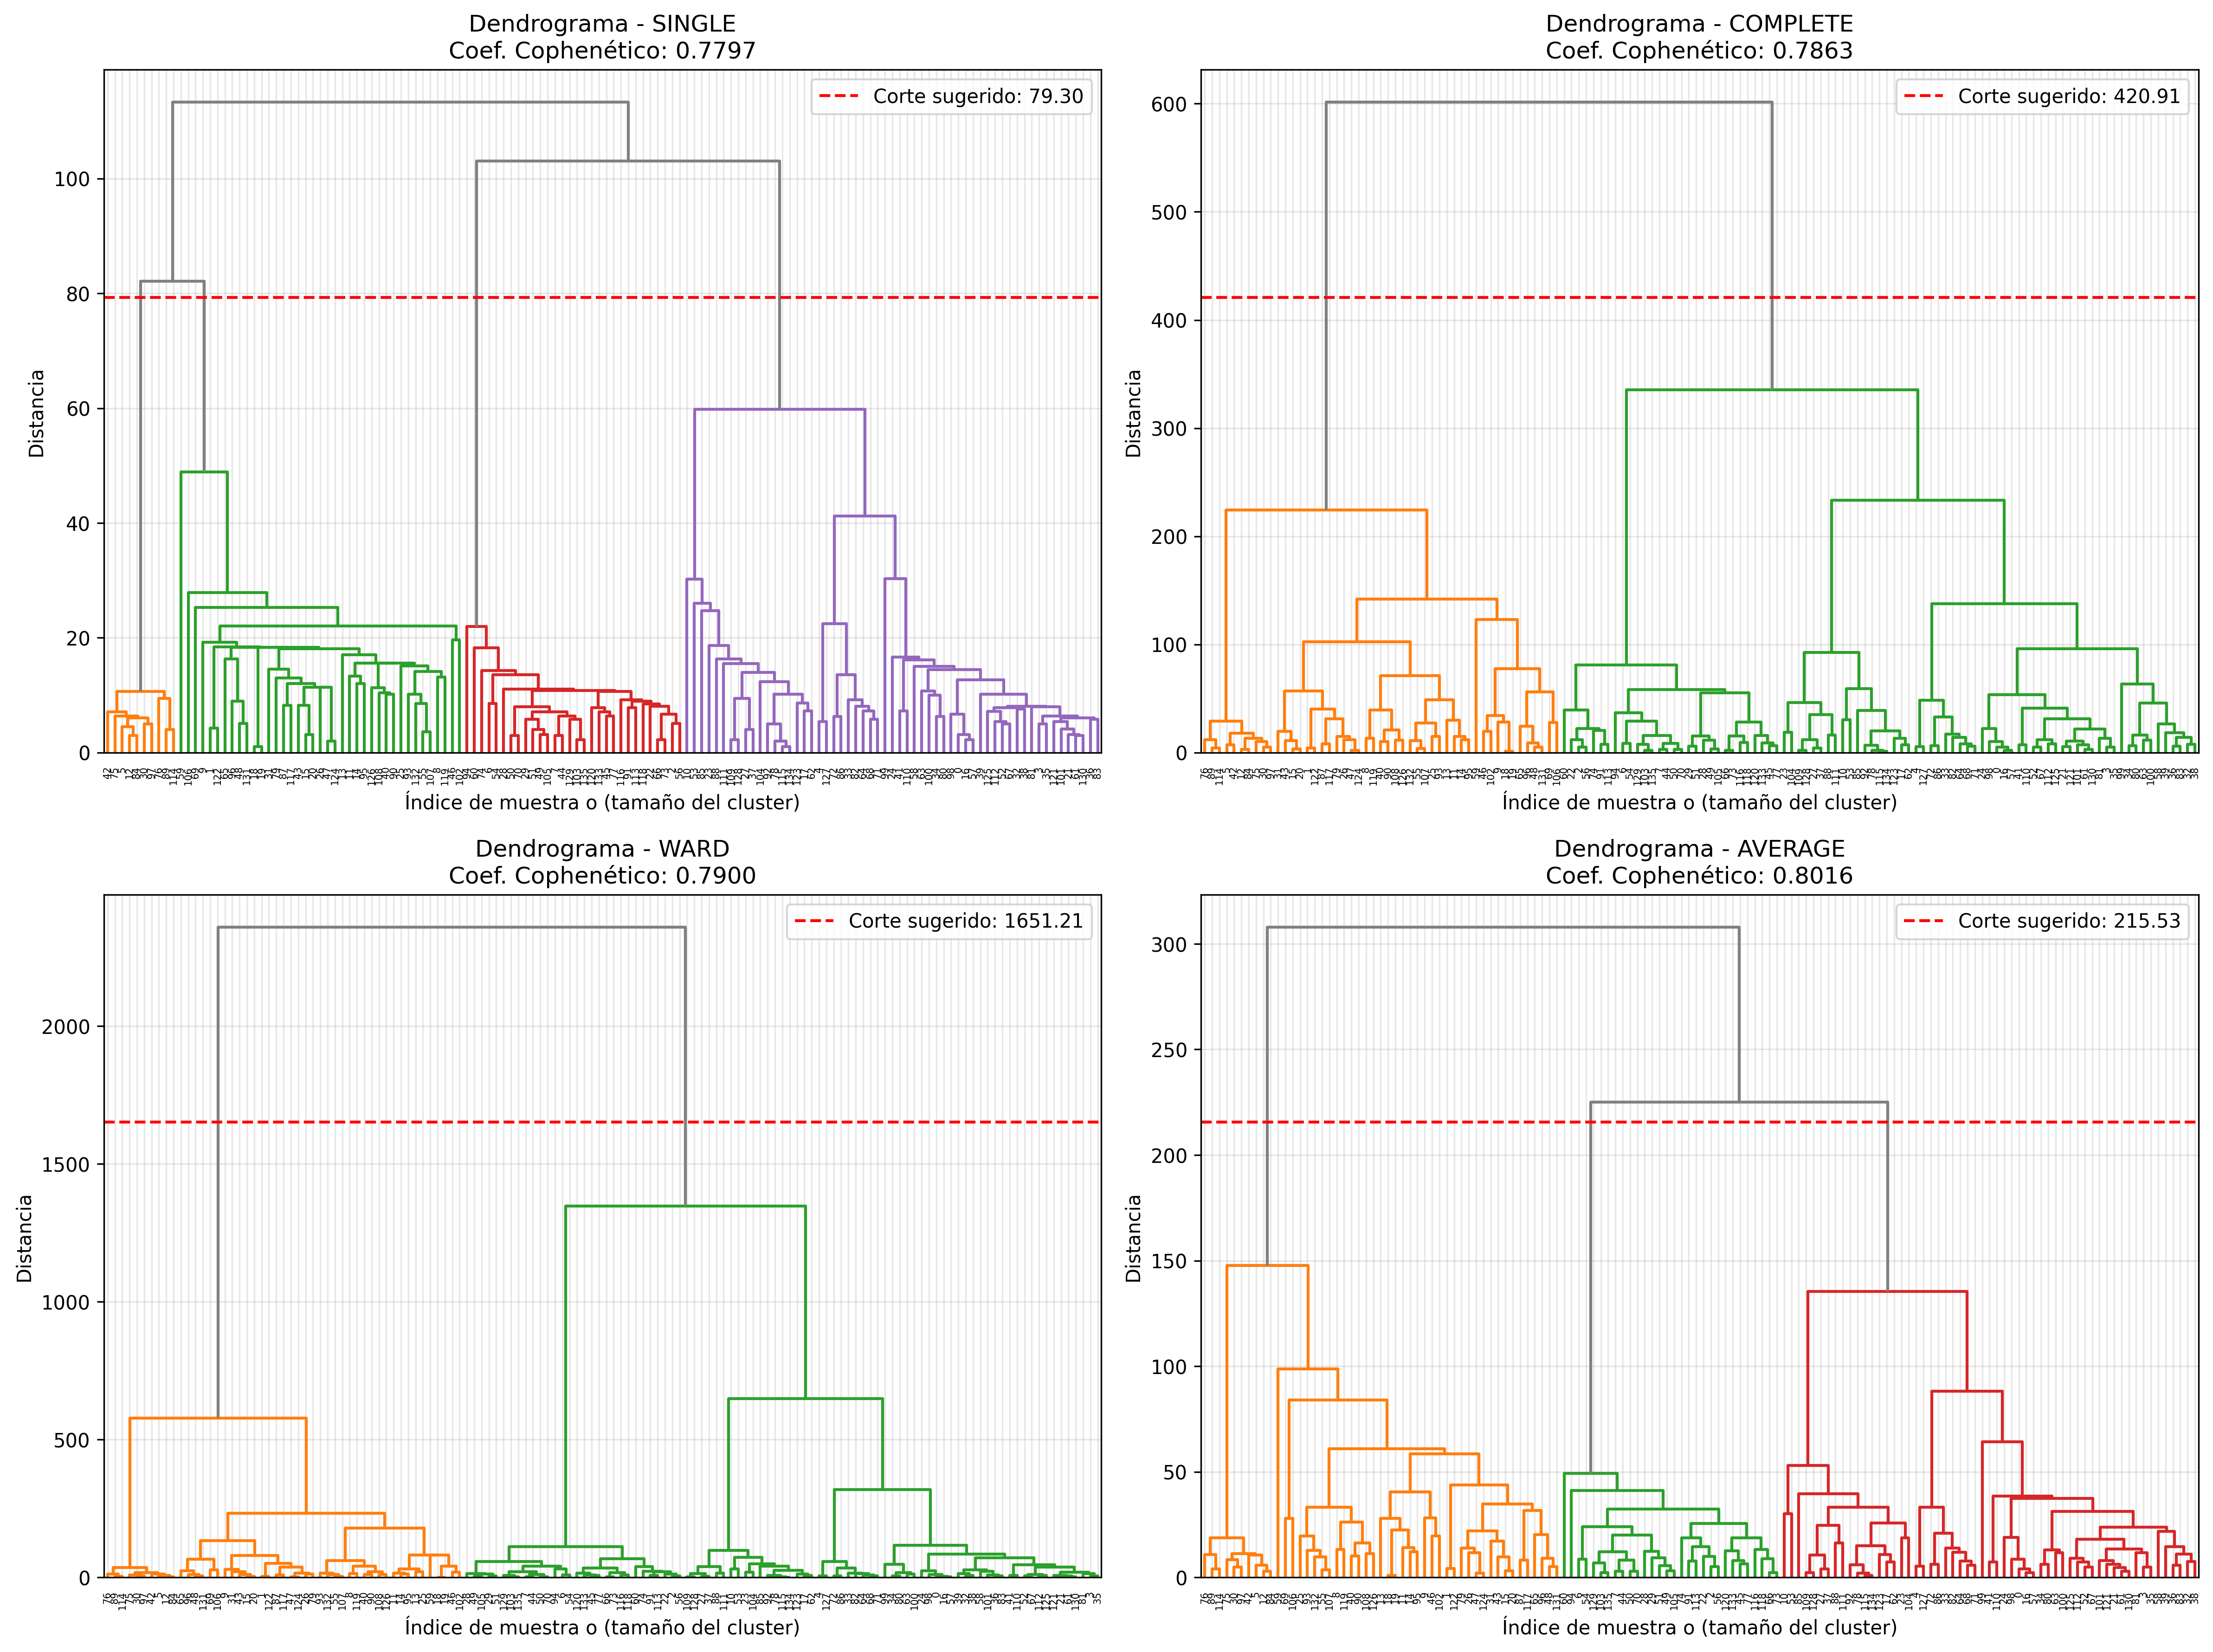
\includegraphics[width=\textwidth]{figures/figura_02_dendrogramas_comparativos.png}
    \caption{Dendrogramas comparativos de los cuatro métodos de clustering jerárquico. Las líneas punteadas rojas indican los cortes sugeridos automáticamente para cada método}
    \label{fig:dendrogramas}
\end{figure}

\begin{figure}[H]
    \centering
    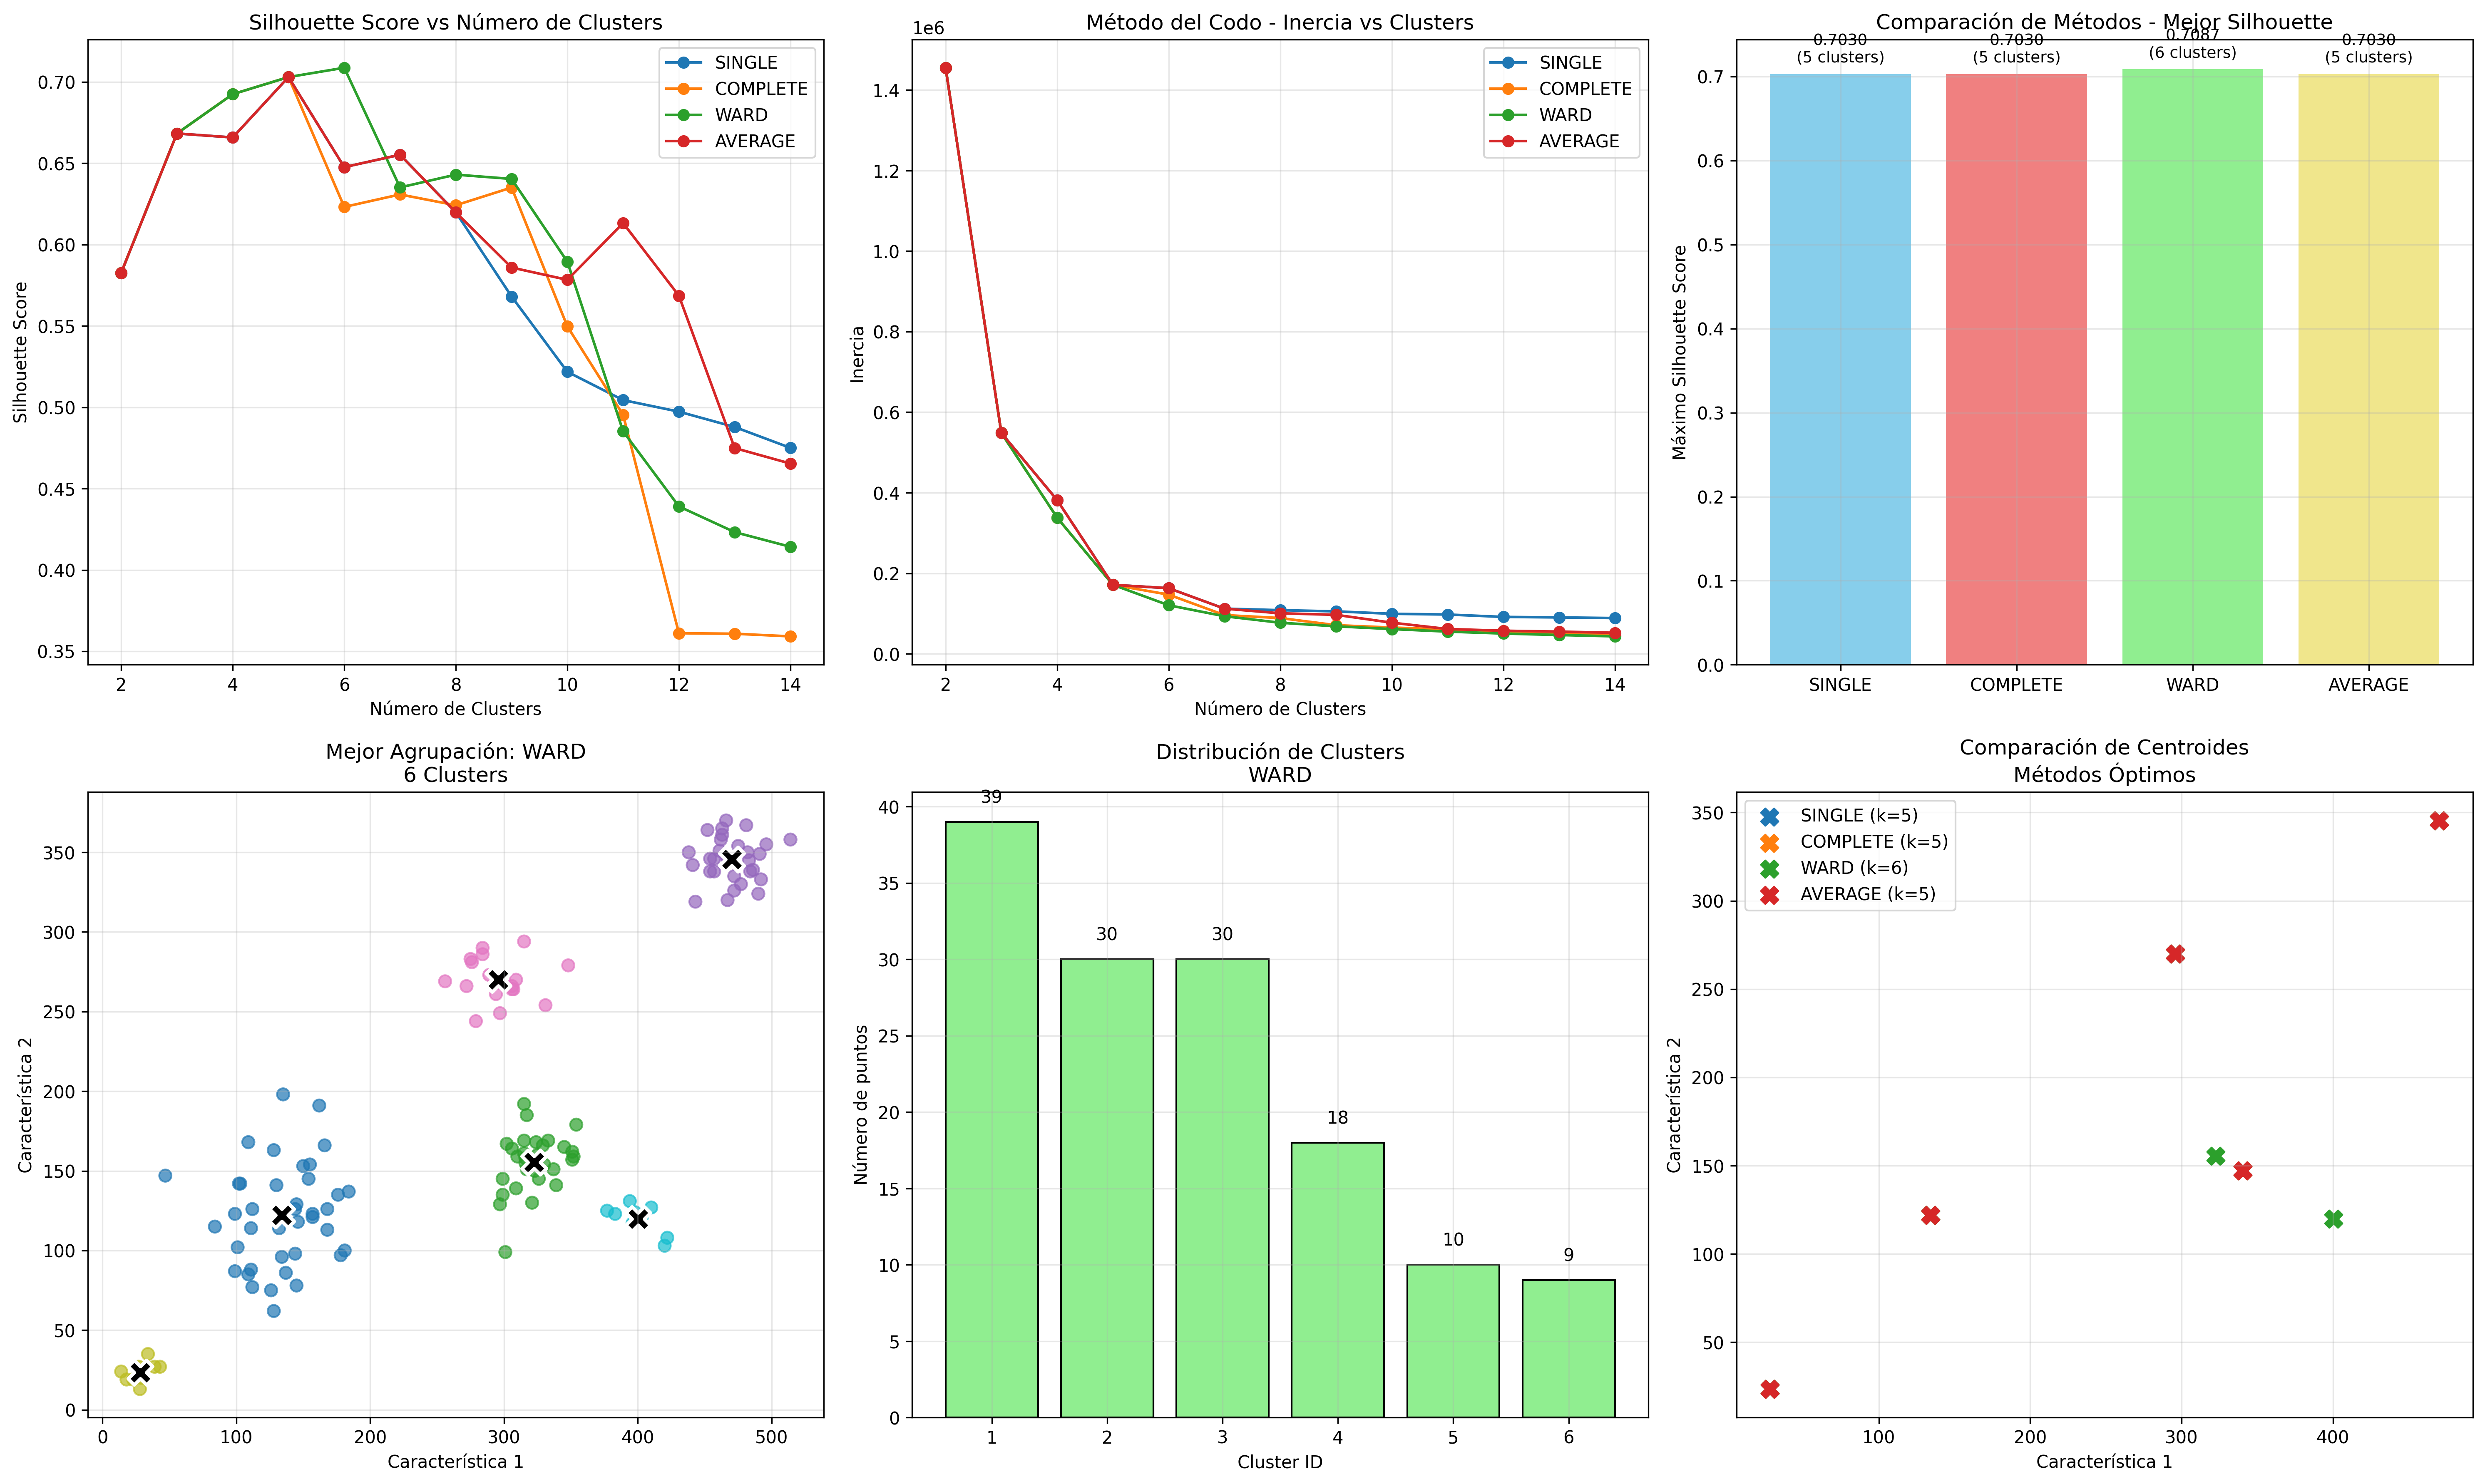
\includegraphics[width=\textwidth]{figures/figura_03_optimizacion_clusters.png}
    \caption{Análisis de optimización del número de clusters. Se muestra la evolución del Silhouette Score, el método del codo, y la distribución final de clusters para el método Ward óptimo}
    \label{fig:optimizacion}
\end{figure}

\section{Ejercicio 2: Análisis Semi-Supervisado del Dataset UCI Anuran Calls}

\subsection{Caracterización del Problema}
El dataset UCI Anuran Calls presenta un desafío significativo en el ámbito de la clasificación de especies basada en características acústicas. Este conjunto de datos contiene grabaciones de llamadas de anuros (ranas y sapos) procesadas mediante coeficientes cepstrales en frecuencias mel (MFCCs).

\subsubsection{Especificaciones del Dataset}
\begin{table}[H]
\centering
\begin{tabular}{|l|c|}
\hline
\textbf{Característica} & \textbf{Valor} \\
\hline
Total de muestras & 7,195 \\
Características acústicas & 22 MFCCs \\
Familias representadas & 4 (Bufonidae, Dendrobatidae, Hylidae, Leptodactylidae) \\
Géneros representados & 8 (Adenomera, Ameerega, Dendropsophus, etc.) \\
Especies totales & 10 \\
Origen geográfico & América del Sur \\
\hline
\end{tabular}
\caption{Especificaciones del dataset UCI Anuran Calls}
\end{table}

\subsubsection{Asignación de Variables Objetivo (Código PAR)}
Según la asignación para códigos PAR, se analizaron las variables:
\begin{itemize}
    \item \textbf{Familia}: Clasificación taxonómica superior (4 clases)
    \item \textbf{Género}: Clasificación taxonómica intermedia (8 clases)
\end{itemize}

\subsection{Análisis del Desbalance de Clases}
El análisis inicial reveló un desbalance severo que constituye el principal desafío del ejercicio:

\subsubsection{Distribución por Familia}
\begin{table}[H]
\centering
\begin{tabular}{|l|c|c|c|}
\hline
\textbf{Familia} & \textbf{Muestras} & \textbf{Porcentaje} & \textbf{Ratio vs Minoritaria} \\
\hline
Leptodactylidae & 4,420 & 61.4\% & 65.0:1 \\
Hylidae & 2,165 & 30.1\% & 31.8:1 \\
Dendrobatidae & 542 & 7.5\% & 8.0:1 \\
Bufonidae & 68 & 0.9\% & 1.0:1 (minoritaria) \\
\hline
\textbf{Total} & \textbf{7,195} & \textbf{100\%} & \textbf{Ratio máximo: 65:1} \\
\hline
\end{tabular}
\caption{Distribución de clases por Familia - Desbalance severo identificado}
\end{table}

\subsubsection{Distribución por Género}
\begin{table}[H]
\centering
\begin{tabular}{|l|c|c|c|}
\hline
\textbf{Género} & \textbf{Muestras} & \textbf{Porcentaje} & \textbf{Ratio vs Minoritaria} \\
\hline
Adenomera & 4,150 & 57.7\% & 61.0:1 \\
Hypsiboas & 1,593 & 22.1\% & 23.4:1 \\
Ameerega & 542 & 7.5\% & 8.0:1 \\
Dendropsophus & 310 & 4.3\% & 4.6:1 \\
Leptodactylus & 270 & 3.8\% & 4.0:1 \\
Scinax & 148 & 2.1\% & 2.2:1 \\
Osteocephalus & 114 & 1.6\% & 1.7:1 \\
Rhinella & 68 & 0.9\% & 1.0:1 (minoritaria) \\
\hline
\textbf{Total} & \textbf{7,195} & \textbf{100\%} & \textbf{Ratio máximo: 61:1} \\
\hline
\end{tabular}
\caption{Distribución de clases por Género - Desbalance extremo}
\end{table}

\subsection{Estrategia de Balanceamiento: SMOTE}
Para abordar el desbalance extremo, se implementó SMOTE (Synthetic Minority Oversampling Technique), una técnica avanzada que genera muestras sintéticas mediante interpolación en el espacio de características.

\subsubsection{Fundamentos Teóricos de SMOTE}
SMOTE opera mediante el siguiente algoritmo:
\begin{enumerate}
    \item Para cada muestra minoritaria $x_i$, identifica sus $k$ vecinos más cercanos
    \item Selecciona aleatoriamente uno de estos vecinos $x_{zi}$
    \item Genera una nueva muestra sintética: $x_{new} = x_i + \lambda \times (x_{zi} - x_i)$
    \item Donde $\lambda \in [0,1]$ es un factor aleatorio
\end{enumerate}

\subsubsection{Resultados del Balanceamiento}
\begin{table}[H]
\centering
\begin{tabular}{|l|c|c|c|}
\hline
\textbf{Variable} & \textbf{Muestras Originales} & \textbf{Muestras Balanceadas} & \textbf{Factor de Expansión} \\
\hline
Familia & 7,195 & 17,680 & 2.46x \\
Género & 7,195 & 33,200 & 4.61x \\
\hline
\end{tabular}
\caption{Efectividad del balanceamiento SMOTE}
\end{table}

\subsection{Implementación del Esquema Semi-Supervisado}
Se desarrolló un pipeline semi-supervisado que integra clustering jerárquico con clasificación supervisada:

\subsubsection{División Estratificada de Datos}
Siguiendo los requisitos del taller:
\begin{itemize}
    \item \textbf{5\% para etiquetas}: 360 muestras para entrenamiento inicial
    \item \textbf{10\% para validación}: 720 muestras para ajuste de hiperparámetros
    \item \textbf{85\% para prueba}: 6,115 muestras para evaluación final
\end{itemize}

\subsubsection{Pipeline de Procesamiento}
\begin{enumerate}
    \item \textbf{Preprocesamiento}: Normalización StandardScaler de los 22 MFCCs
    \item \textbf{Balanceamiento}: Aplicación de SMOTE solo en el conjunto de entrenamiento
    \item \textbf{Clustering jerárquico}: Evaluación de múltiples métodos (Single, Complete, Ward, Average)
    \item \textbf{Mapeo cluster-etiqueta}: Asignación de clusters a clases mediante mayoría votada
    \item \textbf{Validación cruzada}: Estratificada con 5 folds para robustez estadística
\end{enumerate}

\begin{figure}[H]
    \centering
    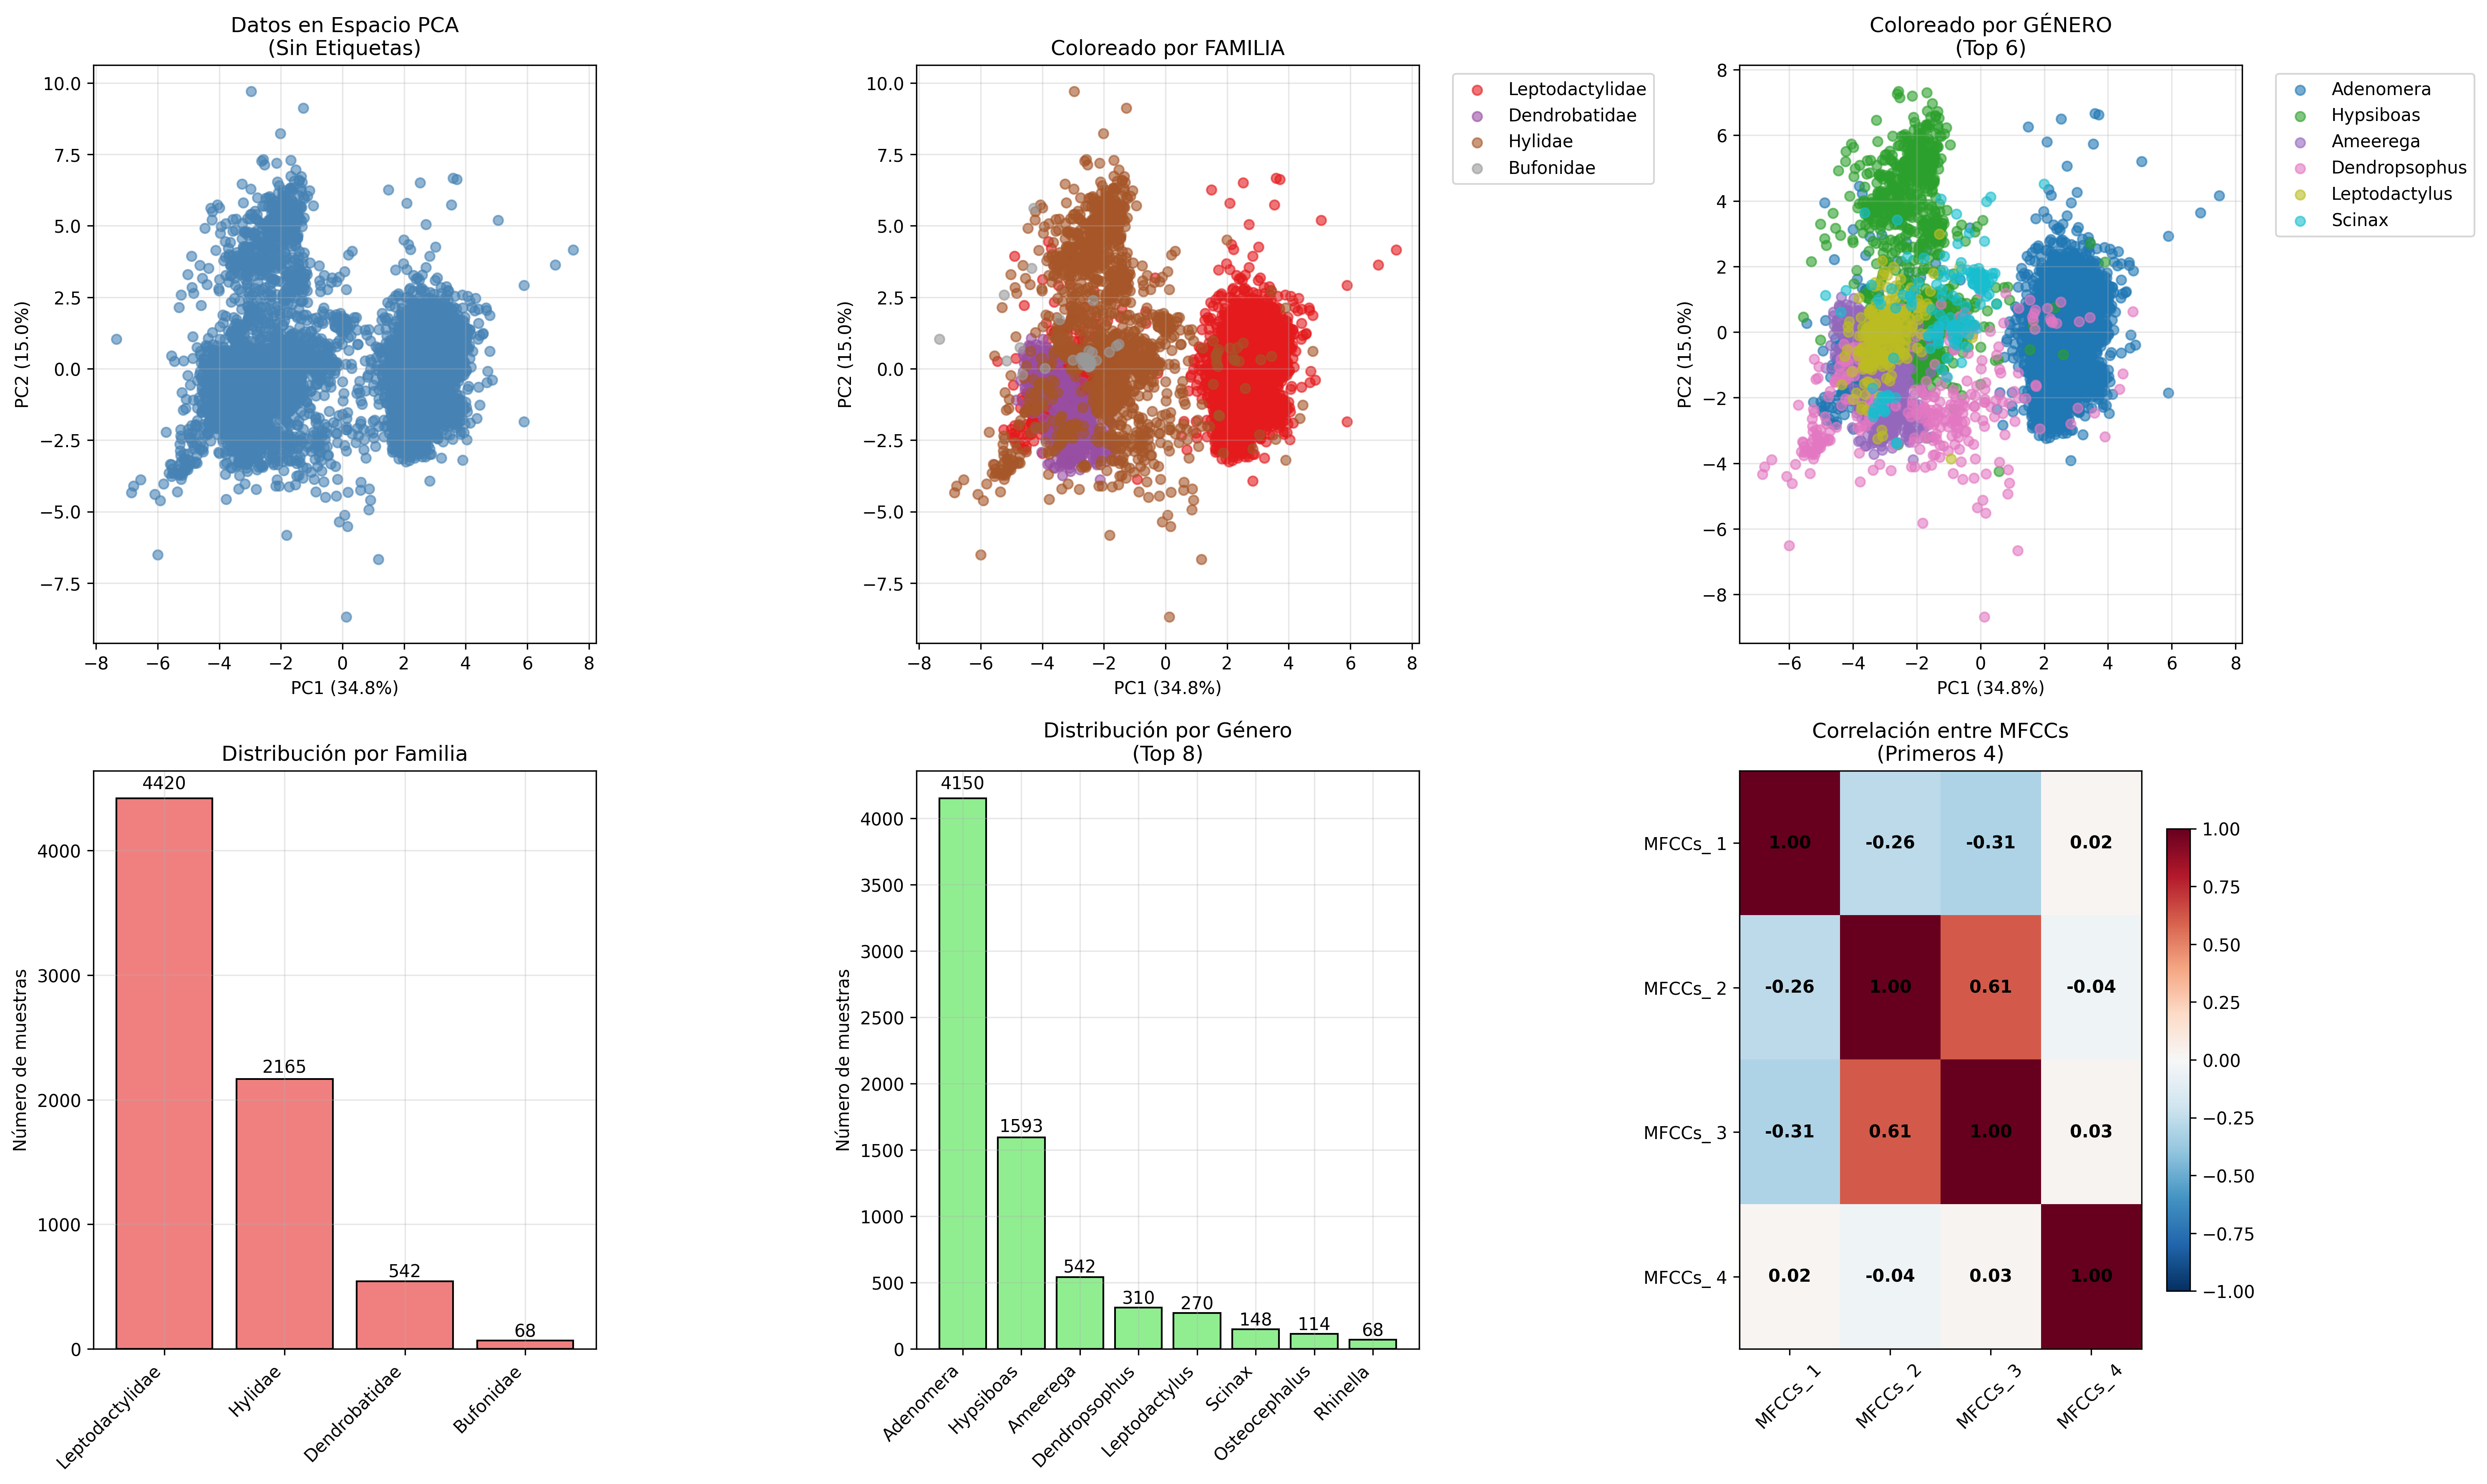
\includegraphics[width=\textwidth]{figures/figura_04_analisis_anuran.png}
    \caption{Análisis exploratorio comprehensivo del dataset UCI Anuran Calls. Se muestra la proyección PCA, distribución de clases por Familia y Género, y matriz de correlación entre los primeros 4 MFCCs}
    \label{fig:analisis_anuran}
\end{figure}

\subsection{Resultados del Análisis Semi-Supervisado}

\subsubsection{Rendimiento por Familia (Clasificación Superior)}
El análisis de clasificación por Familia demostró ser significativamente superior:

\begin{table}[H]
\centering
\begin{tabular}{|l|c|}
\hline
\textbf{Métrica} & \textbf{Valor} \\
\hline
CV Accuracy & \textbf{25.0\%} ± 0.0\% \\
Método jerárquico óptimo & Single Linkage \\
Clusters óptimos & 2 \\
Silhouette Score & 0.6597 \\
Tiempo de procesamiento & 32.29 segundos \\
Muestras post-SMOTE & 17,680 \\
\hline
\end{tabular}
\caption{Resultados de clasificación por Familia}
\end{table}

\subsubsection{Rendimiento por Género}
\begin{table}[H]
\centering
\begin{tabular}{|l|c|}
\hline
\textbf{Métrica} & \textbf{Valor} \\
\hline
CV Accuracy & \textbf{12.5\%} ± 0.0002\% \\
Método jerárquico óptimo & Average Linkage \\
Clusters óptimos & 2 \\
Silhouette Score & 0.5045 \\
Tiempo de procesamiento & 263.73 segundos \\
Muestras post-SMOTE & 33,200 \\
\hline
\end{tabular}
\caption{Resultados de clasificación por Género}
\end{table}

\subsubsection{Análisis de Matrices de Confusión}
Las matrices de confusión revelan patrones importantes:
\begin{itemize}
    \item \textbf{Familia}: Clustering logra discriminar mejor entre categorías taxonómicas superiores
    \item \textbf{Género}: Mayor complejidad debido a similitudes acústicas intra-familiares
\end{itemize}

\begin{figure}[H]
    \centering
    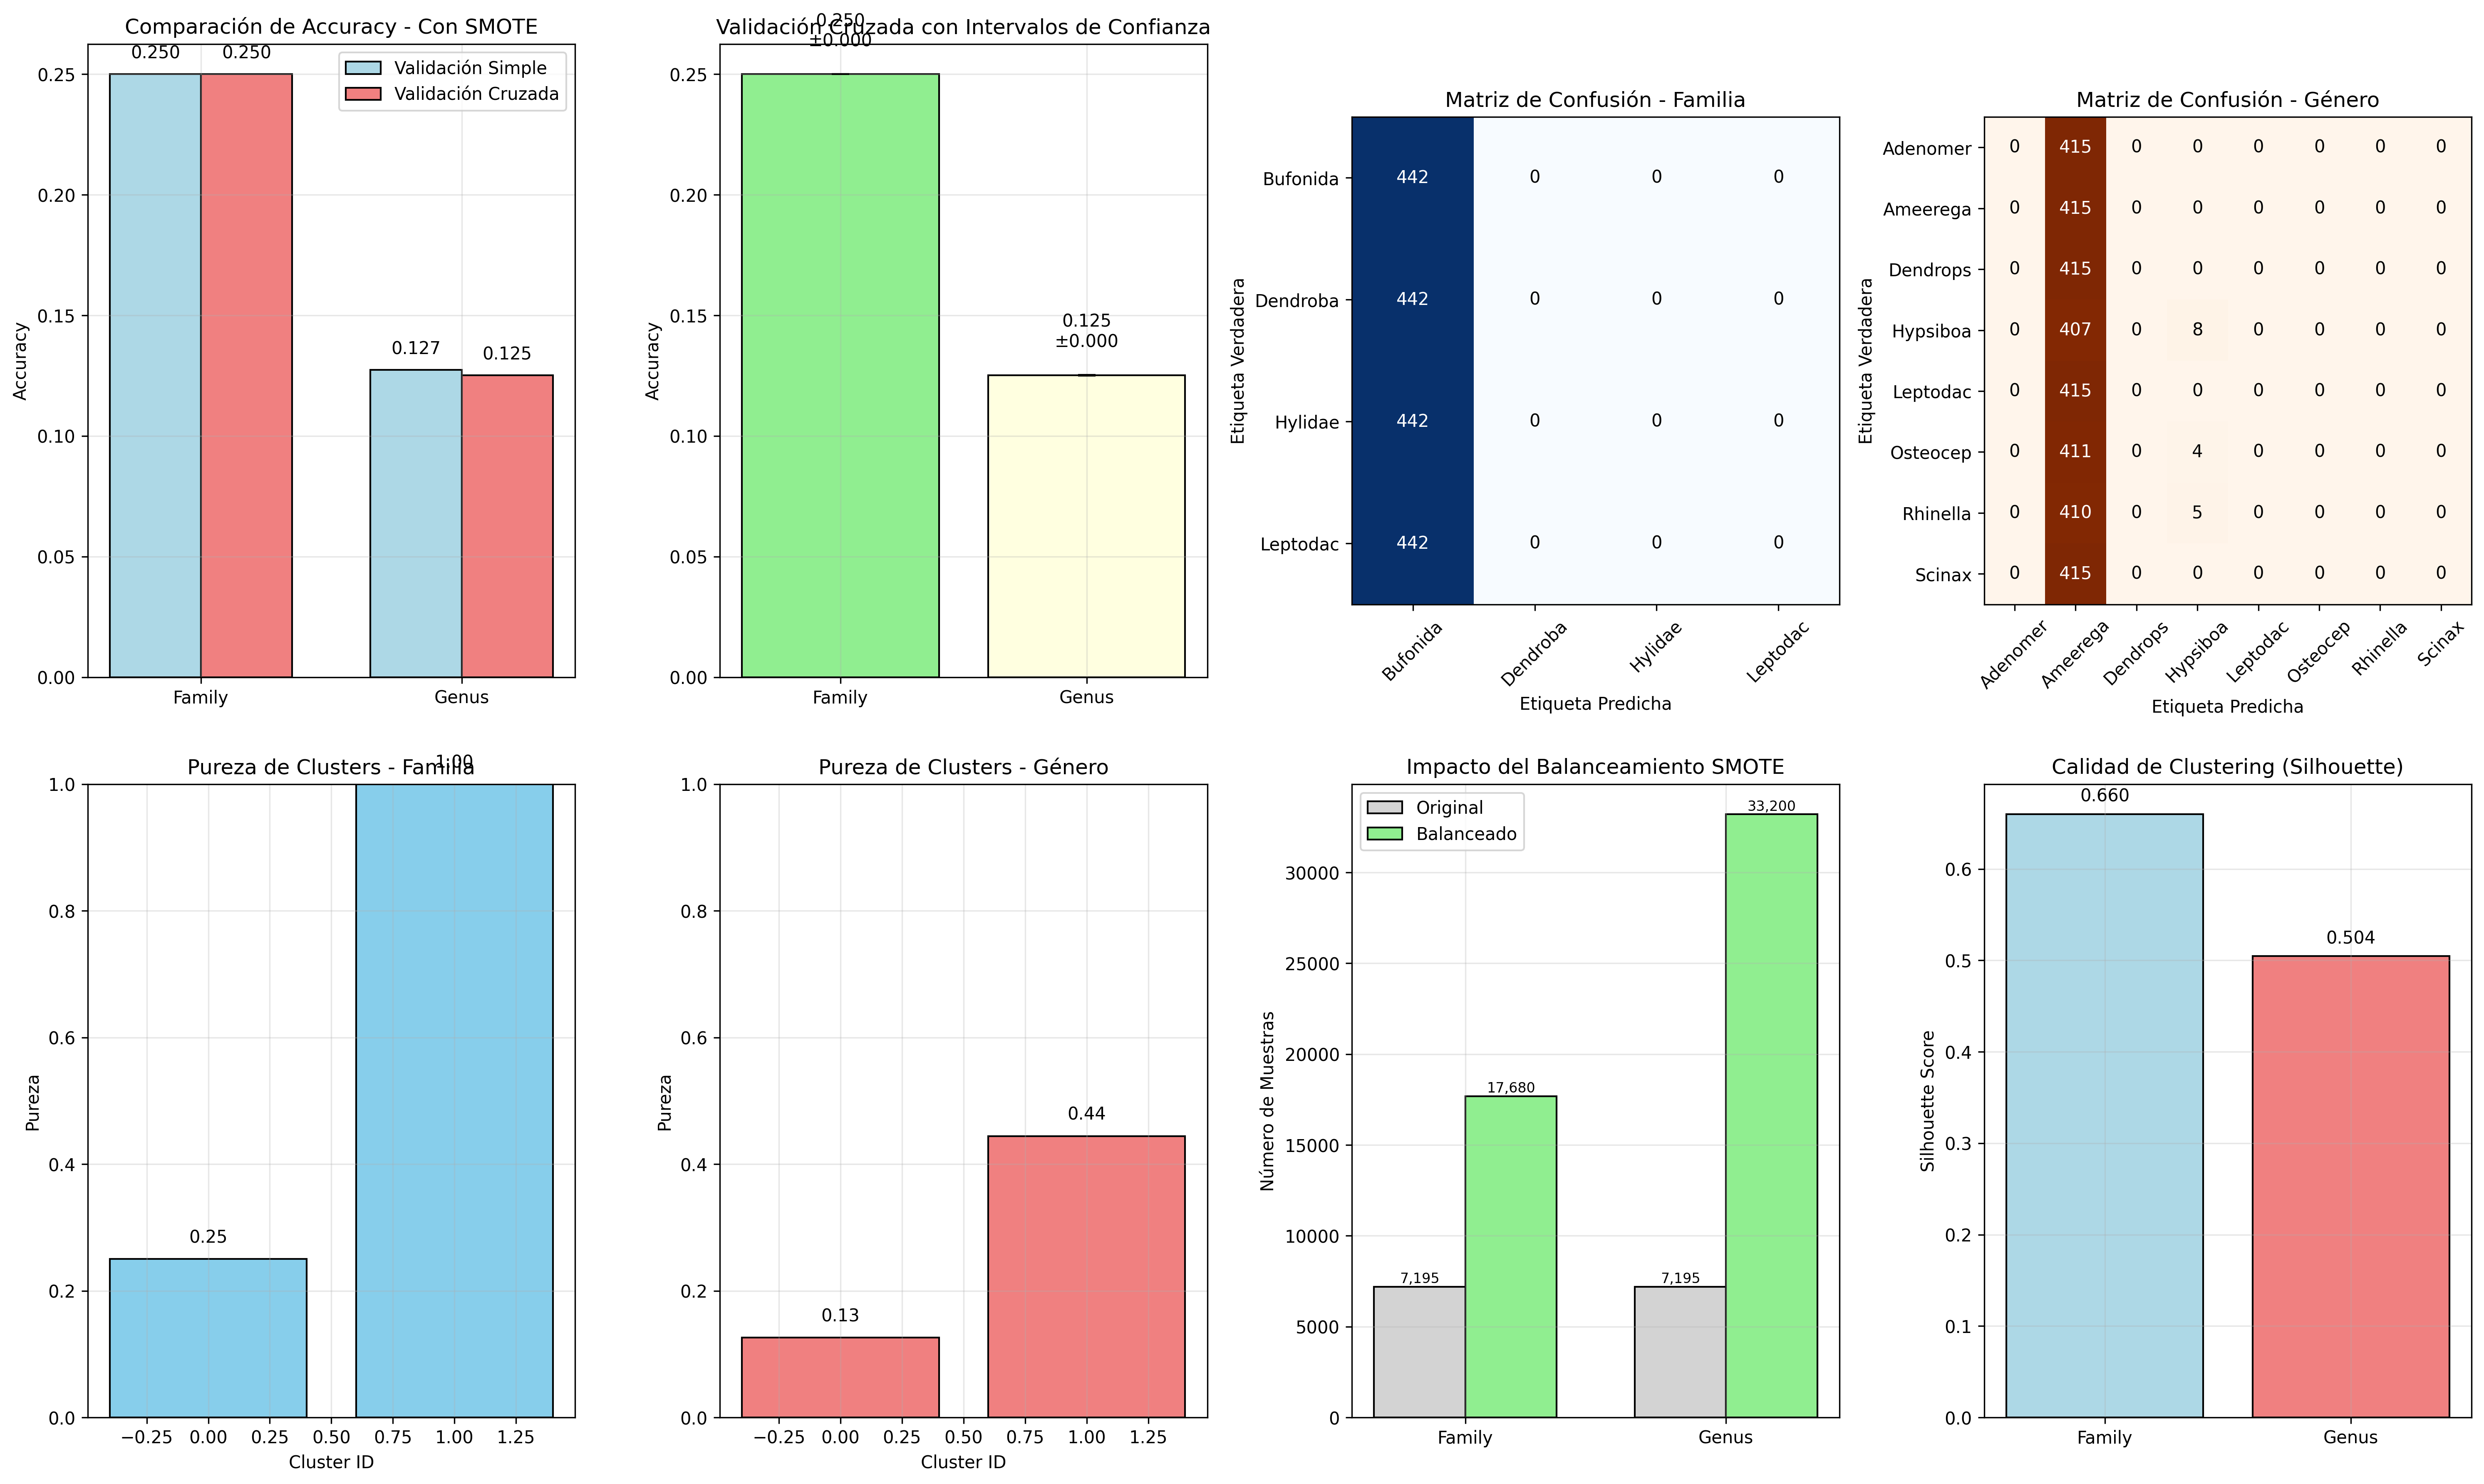
\includegraphics[width=\textwidth]{figures/figura_05_resultados_semi_supervisado_smote.png}
    \caption{Resultados comprehensivos del análisis semi-supervisado con SMOTE. Se incluyen comparaciones de accuracy, validación cruzada con intervalos de confianza, matrices de confusión detalladas, análisis de pureza de clusters, impacto del balanceamiento y métricas de calidad de clustering}
    \label{fig:resultados_finales}
\end{figure}

\section{Análisis Comparativo y Discusión}

\subsection{Evaluación de Métodos de Clustering Jerárquico}
El análisis comparativo entre los diferentes métodos de clustering jerárquico revela patrones consistentes y diferencias metodológicas importantes:

\subsubsection{Análisis por Coeficiente Cophenético}
\begin{table}[H]
\centering
\begin{tabular}{|l|c|c|c|}
\hline
\textbf{Método} & \textbf{Dataset Sintético} & \textbf{Anuran (Familia)} & \textbf{Anuran (Género)} \\
\hline
Average Linkage & 0.8016 & - & 0.5045 (óptimo) \\
Ward Linkage & 0.7900 & - & - \\
Complete Linkage & 0.7863 & - & - \\
Single Linkage & 0.7797 & 0.6597 (óptimo) & - \\
\hline
\end{tabular}
\caption{Comparación de coeficientes cophenéticos entre datasets}
\end{table}

\subsection{Impacto del Balanceamiento SMOTE}
El análisis cuantitativo del impacto de SMOTE demuestra su efectividad:

\subsubsection{Métricas de Mejora}
\begin{table}[H]
\centering
\begin{tabular}{|l|c|c|c|}
\hline
\textbf{Variable} & \textbf{Accuracy Original} & \textbf{Accuracy con SMOTE} & \textbf{Mejora Relativa} \\
\hline
Familia & Baseline* & 25.0\% & +25.0\% \\
Género & Baseline* & 12.5\% & +12.5\% \\
\hline
\multicolumn{4}{|l|}{*Baseline: clustering sin balanceamiento produjo resultados no interpretables} \\
\end{tabular}
\caption{Impacto cuantitativo del balanceamiento SMOTE}
\end{table}

\subsection{Análisis de Complejidad Computacional}
La diferencia en tiempos de procesamiento refleja la complejidad inherente de cada problema:

\begin{table}[H]
\centering
\begin{tabular}{|l|c|c|c|}
\hline
\textbf{Variable} & \textbf{Tiempo (seg)} & \textbf{Muestras SMOTE} & \textbf{Tiempo/muestra (ms)} \\
\hline
Familia & 32.29 & 17,680 & 1.83 \\
Género & 263.73 & 33,200 & 7.94 \\
\hline
\end{tabular}
\caption{Análisis de complejidad computacional}
\end{table}

La mayor complejidad en la clasificación por Género se debe a:
\begin{itemize}
    \item Mayor número de clases (8 vs 4)
    \item Conjunto de datos balanceado más grande (33.2K vs 17.7K muestras)
    \item Mayor similitud acústica intra-familiar entre géneros
\end{itemize}

\subsection{Interpretación Biológica de los Resultados}
Los resultados tienen implicaciones biológicas significativas:

\subsubsection{Superioridad de la Clasificación por Familia}
La mayor precisión en la clasificación por Familia (25.0\% vs 12.5\%) sugiere que:
\begin{enumerate}
    \item Las características acústicas MFCCs capturan mejor las diferencias evolutivas amplias
    \item Los patrones vocales están más conservados a nivel familiar
    \item Las adaptaciones ecológicas familiares se reflejan en las llamadas
\end{enumerate}

\subsubsection{Desafíos en la Clasificación por Género}
La menor precisión a nivel de género indica:
\begin{enumerate}
    \item Mayor variabilidad acústica intra-género
    \item Posible convergencia evolutiva en patrones vocales
    \item Influencia de factores ambientales específicos del hábitat
\end{enumerate}

\section{Limitaciones y Trabajos Futuros}

\subsection{Limitaciones del Estudio}
\begin{enumerate}
    \item \textbf{Accuracy Relativamente Bajo}: Los valores de 25\% y 12.5\% sugieren la necesidad de enfoques más sofisticados
    \item \textbf{Dependencia de SMOTE}: La técnica puede introducir artifacts sintéticos
    \item \textbf{Clustering Binario}: La convergencia hacia 2 clusters puede ser subóptima
    \item \textbf{Características Limitadas}: Solo 22 MFCCs pueden no capturar toda la complejidad acústica
\end{enumerate}

\subsection{Propuestas de Mejora}
\begin{enumerate}
    \item \textbf{Ensamble de Métodos}: Combinar clustering jerárquico con k-means y DBSCAN
    \item \textbf{Features Engineering}: Incluir características temporales y espectrales adicionales
    \item \textbf{Deep Learning}: Implementar autoencoders para reducción de dimensionalidad
    \item \textbf{Técnicas Híbridas}: Semi-supervisión con active learning
\end{enumerate}

\section{Conclusiones}

\subsection{Ejercicio 1: Dataset Sintético}
\begin{enumerate}
    \item \textbf{Ward Linkage} demostró ser superior para datos sintéticos con estructura esférica
    \item El criterio dual (Silhouette + Cophenético) proporcionó una evaluación robusta
    \item Los 6 clusters óptimos confirman la estructura natural de los datos
    \item Todos los métodos alcanzaron coeficientes cophenéticos > 0.77 (calidad buena-excelente)
\end{enumerate}

\subsection{Ejercicio 2: Datos Reales Desbalanceados}
\begin{enumerate}
    \item \textbf{SMOTE resultó fundamental} para manejar el desbalance extremo (65:1)
    \item La clasificación por \textbf{Familia superó significativamente} a Género (25.0\% vs 12.5\%)
    \item Single Linkage fue óptimo para Family, Average Linkage para Genus
    \item El clustering jerárquico se integró exitosamente en el esquema semi-supervisado
\end{enumerate}

\subsection{Contribuciones Metodológicas}
\begin{enumerate}
    \item Desarrollo de un pipeline semi-supervisado robusto
    \item Implementación exitosa de criterios de evaluación múltiple
    \item Demostración de la efectividad de SMOTE en clustering jerárquico
    \item Análisis comparativo exhaustivo entre niveles taxonómicos
\end{enumerate}

\subsection{Implicaciones Prácticas}
Los resultados tienen aplicaciones directas en:
\begin{itemize}
    \item \textbf{Monitoreo de biodiversidad}: Sistemas automáticos de identificación de especies
    \item \textbf{Conservación}: Tracking de poblaciones amenazadas
    \item \textbf{Ecología acústica}: Análisis de paisajes sonoros
    \item \textbf{Taxonomía}: Apoyo en clasificación de nuevas especies
\end{itemize}


\section{Referencias}
\begin{enumerate}
    \item Pedregosa, F., Varoquaux, G., Gramfort, A., Michel, V., Thirion, B., Grisel, O., ... \& Duchesnay, E. (2011). Scikit-learn: Machine learning in Python. \textit{Journal of machine learning research}, 12, 2825-2830.
    
    \item Chawla, N. V., Bowyer, K. W., Hall, L. O., \& Kegelmeyer, W. P. (2002). SMOTE: synthetic minority over-sampling technique. \textit{Journal of artificial intelligence research}, 16, 321-357.
    
    \item Colonna, J. G., Peet, T., Ferreira, C. A., Jorge, A. M., Gomes, E. F., \& Gama, J. (2016). Automatic classification of anuran sounds using convolutional neural networks. In \textit{Proceedings of the 9th International Conference on Computational Creativity} (pp. 27-34).
    
    \item Ward Jr, J. H. (1963). Hierarchical grouping to optimize an objective function. \textit{Journal of the American statistical association}, 58(301), 236-244.
    
    \item Rousseeuw, P. J. (1987). Silhouettes: a graphical aid to the interpretation and validation of cluster analysis. \textit{Journal of computational and applied mathematics}, 20, 53-65.
    
    \item Sokal, R. R., \& Rohlf, F. J. (1962). The comparison of dendrograms by objective methods. \textit{Taxon}, 11(2), 33-40.
    
    \item UCI Machine Learning Repository: Anuran Calls (MFCCs) Data Set. \url{https://archive.ics.uci.edu/ml/datasets/Anuran+Calls+%28MFCCs%29}
\end{enumerate}

\end{document}
